\documentclass{article}
\usepackage[polish]{babel}
\usepackage[T1]{fontenc}
\usepackage[utf8]{inputenc}
\usepackage{polski}   
\usepackage{graphicx}   % rysunki
\usepackage{listings}   % kody programów
\usepackage{enumerate}
\usepackage{listings}

\def\TytulPolski {Mobilna gra Lau Kata Kati}

\def\Students {Piotr Maleszczuk\\Łukasz Błaszczak\\Przemysław Burdelak}

%Kierunek:
\def\Kierunek {Informatyka}
 
%Specjalnosc:
\def\Specjalnosc {Technologie informatyczne}

%Poziom studiów: 
\def\PoziomStudiow {I stopnia}

%Forma studiów:
\def\FormaStudiow {stacjonarne}      

%Przedmiot
\def\Przedmiot {Wybrane technologie internetowe}

% Zmiana nazw w opisie tabel i rysunków
\AtBeginDocument{
    \renewcommand*{\tablename}{Tabela}
    \renewcommand*{\figurename}{Rys.} 
}
        




\title{\TytulPolski}
\author{\Student}

\begin{document}
\thispagestyle{empty}
\begin{center}\LARGE
	Politechnika Poznańska\\
	Wydział Elektryczny\\  
	Instytut Automatyki i Inżynierii Informatycznej\\
	  \vspace{15mm}
	\begin{figure}[ht!]
	  	\centering
	  	
\includegraphics[width=50mm]{img/pplogo.png}
	\end{figure}
	  \vspace{15mm}
	\large{\Students}\\
	  \vspace{15mm}
	\LARGE\textbf{\TytulPolski}\\
\end{center}

\begin{center}\vfill
	Poznań, 2017
\end{center} % strona tytułowa
\newpage\tableofcontents    % spis treści
\newpage\section{Wstęp}
\subsection{Opis tematu}
Realizacja gry Lau Kata Kati, polegająca na utworzeniu ogólnej architektury gry pozwalającej na przeprowadzenie rozgrywki zgodnie z zasadami, a następnie podłączenie maszyny grającej, która rywalizuje z użytkownikiem.\\

\subsection{Założenia realizacyjne}
Aplikacja przeznaczona na urządzenia mobilne z system Android w wersji minimum 4.0.3. Do implementacji gry został wykorzystany silnik Unity 5.5.2f1, który zapewnia szeroką gamę narzędzi potrzebnych do napisania kompletnej gry, tj. graficzny interfejs zarządzania sceną, pisanie skryptów w języku C\# obsługujących poszczególny elementy gry, budowanie aplikacji na urządzenia Android. Do pisania skryptów wykorzystano środowisko Visual Studio.\\
\\
Maszyna grająca swoje działanie opiera na strategii Minimax z Alfa-Beta cięciami. Algorytm pobiera aktualny stan planszy w postaci tablicy dwuwymiarowej, a następnie oblicza najlepszą ścieżkę do określonej głębokości drzewa za pomocą rekurencyjnej metody. Ścieżka wybierana jest na podstawie zysku punktów (punkty maszyny grającej - punkty gracza). Po wybraniu najlepszej drogi, pobierany jest z niej pierwszy ruch, a następnie wywołuje się metodę imitującą naciśnięcie odpowiedniego pionka i punktu przeznaczenia do którego ma zostać przeniesiony. Sposób, w którym imituje się naciśnięcie danego elementu został wybrany, ponieważ był to najszybszy i najprostszy sposób przemianowania dwuosobowej rozgrywki lokalnej na rozgrywkę ze sztuczną inteligencją.\\
\\
Aplikacja posiada:
\begin{itemize}
	\item Trzy tryby rozgrywki (singleplayer, multiplayer lokalny oraz przez połączenie Bluetooth),
	
	\item zmianę poziomu trudności maszyny grającej,
	
	\item zmianę skórek pionków,
	
	\item system reklam, 
	
	\item system zbierania danych.
\end{itemize}
	        % wstęp     
\newpage\section{Podział i harmonogram pracy}
W rozdziale przedstawiony został podział pracy między autorami projektu \\(Tabela 1). Harmonogram pracy widoczny jest w Tabeli 2.

\begin{table}[!ht]
	\centering
	\begin{tabular}{|c|p{7cm}|}
		\hline \textit{Autor} & \textit{Podzadanie} \\ \hline
		Piotr Maleszczuk & GUI, wizualizacja ruchów, obsługa różnych trybów gry, implementacja metody Minimax \\ \hline
	
		Łukasz Błaszczak & Przygotowanie planszy, obsługa kliknięć ekranu, przeliczanie punktów, imitacja kliknięć \\ \hline
	
		Przemysław Burdelak & Odnajdywanie możliwych ruchów pionka, budowanie dostępnych plansz, podłączenie maszyny grającej do rozgrywki \\ \hline
	\end{tabular}
	\caption{Podział pracy}
\end{table}

\begin{table}[!ht]
	\centering
	\begin{tabular}{|c|p{7cm}|}
		\hline
		\textit{Lp.} & \textit{Opis zadań} \\ \hline
		1. & Przygotowanie zdalnego repozytorium \\ \hline
		2. & Przygotowanie środowiska programistycznego \\ \hline
		3. & Przygotowanie środowiska Unity oraz założenie wstępnego projektu \\ \hline
		4. & Rozpisanie projektu na Trello, podzielenie na poszczególne zadania wykonywane przez cały czas projektu. \\ \hline
		5. & Utworzenie menu startowego gry (ekran główny, opcje, sklep) \\ \hline
		6. & Utworzenie menu wyboru trybu (singleplayer, multiplayer, online multiplayer) \\ \hline
		7. & Implementacja rozgrywki - logika gry \\ \hline
		8. & Implementacja gry jednoosobowej - SI \\ \hline
		9. & Komunikacja Bluetooth \\ \hline
		10. & Implementacja gry wieloosobowej \\ \hline
		11. & System reklam \\ \hline
		12. & System zbierania danych \\ \hline
		13. & Testy i ewentualne poprawki \\ \hline
	\end{tabular}
	\caption{Harmonogram pracy}
\end{table}

		    % podział pracy
\newpage\section{Funkcjonalności oferowane przez aplikację}

\subsection{Rozgrywka singleplayer}
Rozgrywka realizowana z maszyną grającą opierającą się na strategii Minimax z Alfa-Beta cięciami. Tak jak w przypadku każdego trybu na początku losowany jest gracz rozpoczynający grę, następnie odbywa się całość rozgrywki z botem.

\subsection{Rozgrywka multiplayer local}
W tym przypadku mamy możliwość rozegrania gry dwuosobowej na jednym urządzeniu.

\subsection{Rozgrywka multiplayer bluetooth}
Możliwość rozegrania gry dwuosobowej pomiędzy dwoma urządzeniami na których wykonywane są ruchy poszczególnych graczy.

\subsection{Funkcjonalność sklepu}
Gra rozwinięta jest o możliwości zmiany widoku gry, konkretnie chodzi tutaj o wygląd pionków graczy. Wszystkie oferowane w aplikacji pionki możliwe są do obejrzenia w sklepie. Pionki można używać dopiero po wykupieniu ich za wirtualne monety nabywane bezpośrednio w rozgrywce bądź jako nagroda za obejrzenie reklamy wideo w menu (dostępne raz na 20 minut) za 10 wirtualnych monet, wszystkie pionki dostępne są w różnych cenach.

\subsection{Zmiana trudności AI}
Po wejściu w Opcje (“Options”) możliwa jest również zmiana poziomu maszyny grającej, dostępnej w rozgrywce dla jednego gracza, odpowiadająca głębokości przeszukiwania drzewa a algorytmie minimax’a. Maksymalny możliwy poziom do wybrania to ‘9’. % funkcjonalności aplikacji    
\newpage\section{Wybór technologii informatycznych}
W rodziale znajduje się opis wybranych technologii informatycznych. W kolejnych podsekcjach umieszczone zostały szczegółowe opisy technologii.

\subsection{System Latex}
Oprogramowanie przeznaczone do zautomatyzowanego składu tekstu, a także związany z nim język znaczników, służący do formatowania dokumentów tekstowych i tekstowo-graficznych.

\subsection{System Github}
Hostingowy serwis internetowy przeznaczony dla projektów programistycznych wykorzystujących system kontroli wersji Git.  Wybrany ze względu na łatwość \\w użyciu.

\subsection{System Trello}
Narzędzie wykorzystane do zarządzania zadaniami podczas tworzenia projektu. Projekt w całości został rozpisany w systemie na zadania główne, składające się następnie z mniejszych szczegółowych podzadań. Pozwoliło to na przejrzysty\\ i zaplanowany z góry sposób działania.

\subsection{Język programowania C\#}
Język C\# doskonale współpracuje ze środowiskiem Unity.

\subsection{Środowisko programistyczne Visual Studio}
Zintegrowane środowisko programistyczne firmy Microsoft. Jedno z najbardziej rozwiniętych tego typu narzędzie posiadających ze sobą wiele udogodnień. \\Pomimo swojej wielkości dobrze sprawdza się w każdego rodzaju projekcie. \\W porównaniu ze środowiskiem dostarczonym przez Unity (MonoDevelop) jest to narzędzie bardziej stabilne i wygodniejsze w użyciu.

\subsection{Środowisko Unity}
Zintegrowane środowisko firmy Unity Technologies używane do tworzenia gier wideo na PC, konsole, urządzenia mobilne.\\
Wyborem w tym przypadku kierowaliśmy się głównie na podstawie informacji z internetu oraz niewielką znajomością tego narzędzia przez jednego z członków naszego zespołu. Środowisko pomimo tego, że na pierwszy rzut oka może wydawać się bardzo skomplikowane, po krótkim zapoznaniu okazuje się bardzo przyjemne w użyciu, a do tego ogromna ilość materiałów pomocniczych znajdujących się w internecie.		% opis wybranych technologii
\newpage\section{Architektura}
Rozdział opisuje architekturę, która została wykorzystana w projekcie oraz ogólny opis funkcjonalności zaimplementowanych w danym module.

\subsection{Model View Controller}
Wzorzec projektowy służący do organizowania struktury aplikacji posiadających graficzne interfejsy użytkownika. Zastosowanie go w projekcie umożliwia wygodny podział na kontrolery, które przejmują odpowiedzialność na zadaną funkcjonalnością wykonywaną na modelach. Widoki umożliwiają oddzielenie warstwy prezentacji od wszelkich operacji wewnętrznych.

\subsection{Kontroler planszy}
Kontroler odpowiedzialny za stworzenie oraz obsługę macierzy stanu planszy, na której opiera się cała rozgrywka.  Macierz początkowa ma postać:
$$
\left| \begin{array}{ccccccc}
1 & 1 & 1 & -1 & 2 & 2 & 2 \\
1 & 1 & 1 & 0 & 2 & 2 & 2  \\
1 & 1 & 1 & -1 & 2 & 2 & 2 \\
\end{array} \right|
$$\\
-1 - pole nieużywane \\
0 - pole puste \\
1 - pole z pionkiem gracza 1 \\
2 - pole z pionkiem gracza 2

\subsection{Kontroler tur}
Główny kontroler odpowiedzialny za przebieg całej rozgrywki.\\
Odpowiada za zmianę tur graczy, przeliczanie punktów, zakończenie gry. 

\subsection{Kontroler logiki}
Kontroler na podstawie pozycji pionka oraz macierzy planszy zwraca możliwe dla niego ruchy oraz flagę czy dostępne jest kolejne bicie w tej samej turze. 

\subsection{Kontroler wizualizacji}
Jest to kontroler obsługujący wizualizację przebiegu rozgrywki. 
Przeszukuje macierz pozycji pionków - odpowiednik wirtualnej planszy. Gdy kontroler na danej pozycji w macierzy napotka wartość '1' lub '2' ustawia na odpowiadającym jej polu pionek. Jeżeli wartość ta wynosi '0' usuwa pionek z danego pola planszy.\\
\\
Dodatkowo kontroler obsługuje funkcję wyświetlania podpowiedzi możliwych ruchów dla danego pionka po jego naciśnięciu.

\subsection{Kontroler kliknięć}
Pobiera punkt kliknięcia i szuka elementu tj. pionka, pustego pola,\\
który w danym miejscu się znajduje, a następnie przesyła go do kontolera planszy.

\subsection{Kontroler Bluetooth}
Uruchamia moduł bluetooth, zależnie od wybranego trybu jako klient lub\\
serwer. Korzysta ze specjalnego pluginu, który mapuje działanie bluetooth\\
na wbudowaną obsługę połączenia sieciowego w Unity.

\subsection{Kontroler aktora Bluetooth}
W tym kontrolerze, odbywa się główna komunikacja bluetooth pomiędzy\\
klientem a serwerem. Komuinikaty wysyłane są w prostej czterocyfrowej postaci:\\
s t x y \\
,gdzie: \\
s – status komunikatu 1-setup, 2-waiting, 3-transfer \\
t – tura w rozgrywce \\
x – pozycja x kliknięcia \\
y – pozycja y kliknięcia \\

\subsection{Kontroler SI}
Odpowiedzialny za działanie sztucznej inteligencji podczas rozgrywki jednoosobowej. Maszyna grajaca korzysta ze strategi MiniMax z Alfa-Beta cięciami.

\subsection{Kontroler zapisu danych}
Odpowiada za przechowywanie danych użytkownika tj. stan konta, kupione skórki. Dodatkowo umożliwia komunikację pomiędzy scenami.

\subsection{Kontroler gromadzenia danych}
Kontroler zapisuje do pliku informacje na tematy użytkownika: specyfikacja\\ telefonu, lokalizacja, oglądanie reklam, długość korzystania z aplikacji.

\subsection{Kontroler pauzy}
Umożliwia wykonanie pauzy podczas rozgrywki. Umożliwia wyjście do głównego menu, zrestartowanie rozgrywki oraz wznowienie aktualnej.

\subsection{Kontroler końca gry}
Wywoływany po zakończeniu rozgrywki. Uruchamia reklamy, a następnie umożliwia przejście do menu głównego.

\subsection{Kontroler menu}
Odpowiada za działanie całego menu głównego: obsługa sklepu, zmiany ustawień aplikacji, uruchamianie poszczególnych trybów gry.
	% architektura zbudowania
\newpage\section{Instrukcja użytkowania aplikacji}
Aplikacja przeznaczona na urządzenia mobilne z system Android w wersji minimum 4.0.3.

\begin{enumerate}
	\item Po uruchomieniu aplikacji wyśietli się menu głowne(rys.1.).
	\begin{figure}[ht!]
		\centering
		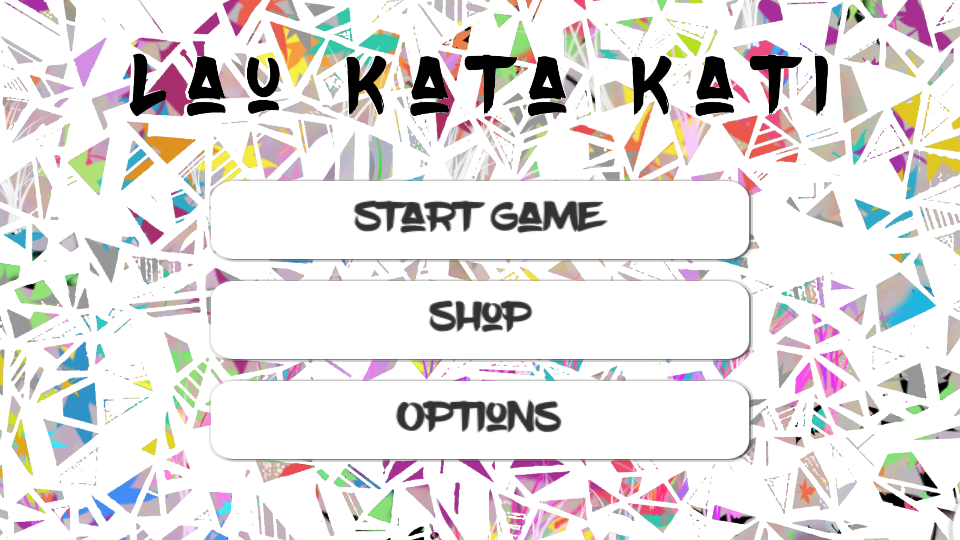
\includegraphics[width=55mm]{img/ekran_glowny.png}
		\caption{Ekran głowny}
	\end{figure}

	\item W menu \textit{„Shop”} istnieje opcja kupna/zmiany skórki pionków za zebrane punkty oraz możliwość obejrzenia reklamy co 20 minut – reklama dodaje 10 punktów (rys.2.).
	\begin{figure}[ht!]
		\centering
		
\includegraphics[width=55mm]{img/sklep.png}
		\caption{Ekran sklepu}
	\end{figure}
	
	\item W menu \textit{„Options"} można ustawić poziom trudności maszyny grającej od 1 do 9 (rys.3.).
	\begin{figure}[ht!]
		\centering
		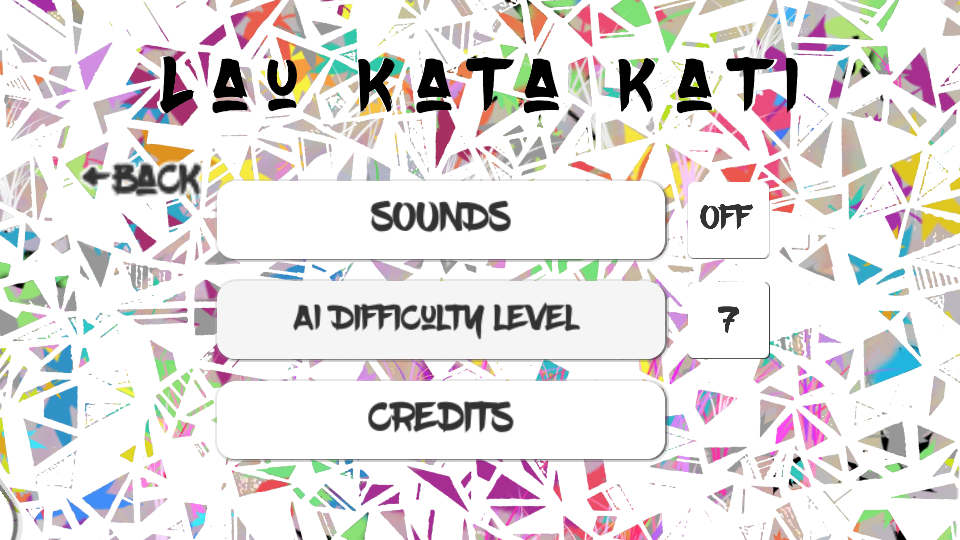
\includegraphics[width=55mm]{img/opcje.png}
		\caption{Ekran opcji}
	\end{figure}
	
	\item Po naciśnięciu \textit{„Start game”} ukażą się trzy tryby rozgrywki (rys.4.):
	\begin{itemize}
		\item \textit{Singleplayer} – rozgrywka przeciwko maszynie grającej,
		\item \textit{Multiplayer} – lokalna rozgrywka dwuosobowa,
		\item \textit{Online Multiplayer} – rozgrywka dwuosobowa przez Bluetooth.
	\end{itemize}
	\begin{figure}[ht!]
		\centering
		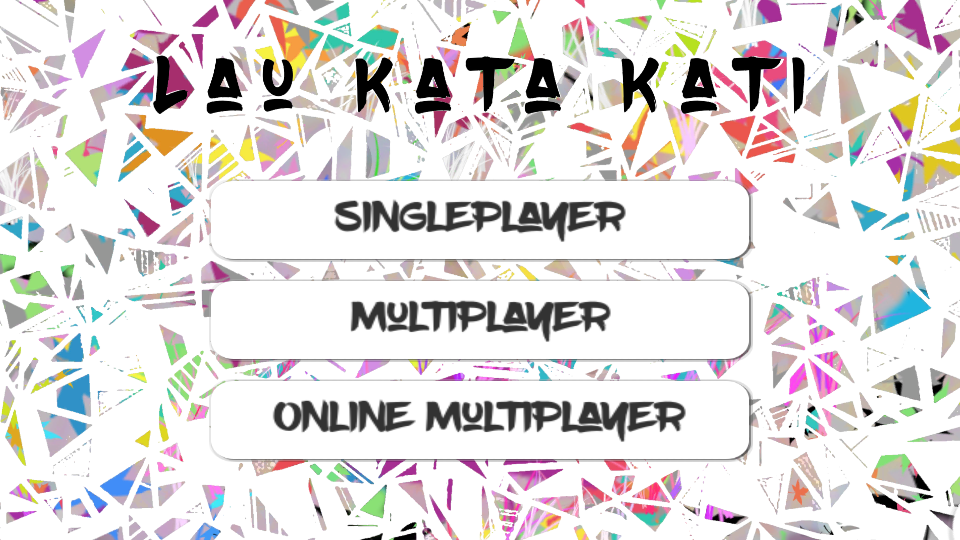
\includegraphics[width=55mm]{img/ekran_trybow.png}
		\caption{Ekran wyboru trybu gry}
	\end{figure}

	\item Po wybraniu trybu \textit{„Singleplayer”} zostanie rozpoczęta rozgrywka przeciwko SI (rys.5.).
	\begin{figure}[ht!]
		\centering
		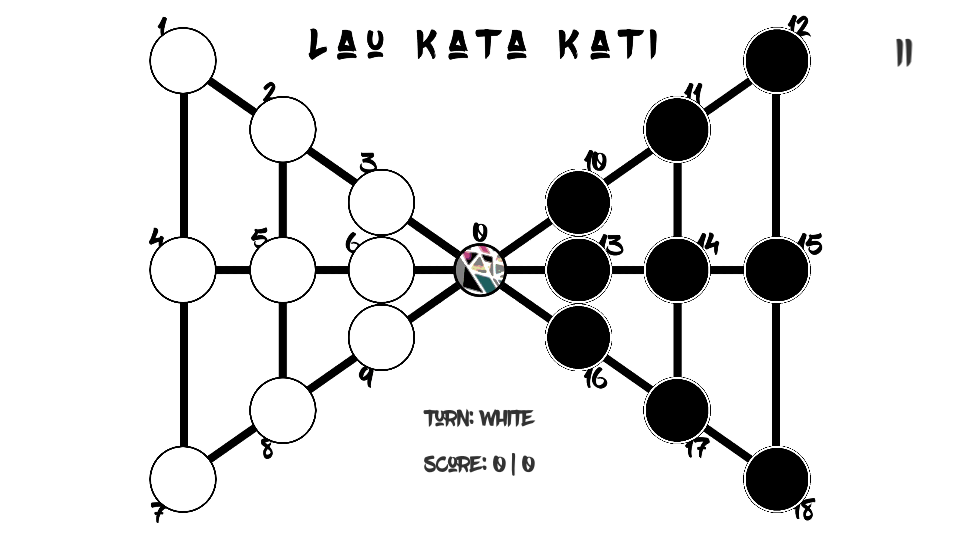
\includegraphics[width=55mm]{img/singleplayer.png}
		\caption{Widok trybu singleplayer}
	\end{figure}

	\item Wybranie trybu \textit{„Multiplayer"} rozpocznie lokalna rozgrywkę multiplayer.
	
	\newpage
	\item Po wybraniu trybu \textit{„Online Multiplayer"} jeden z graczy musi utworzyć serwer gry wybierając opcję \textit{„Server"}. Po utworzeniu serwera gracz drugi łączy się przez Bluetooth wybierając opcję \textit{„Client"}. Rogrywka rozpocznie się po wylosowaniu i przesłaniu tury do klienta (rys.6.). 
	\begin{figure}[ht!]
		\centering
		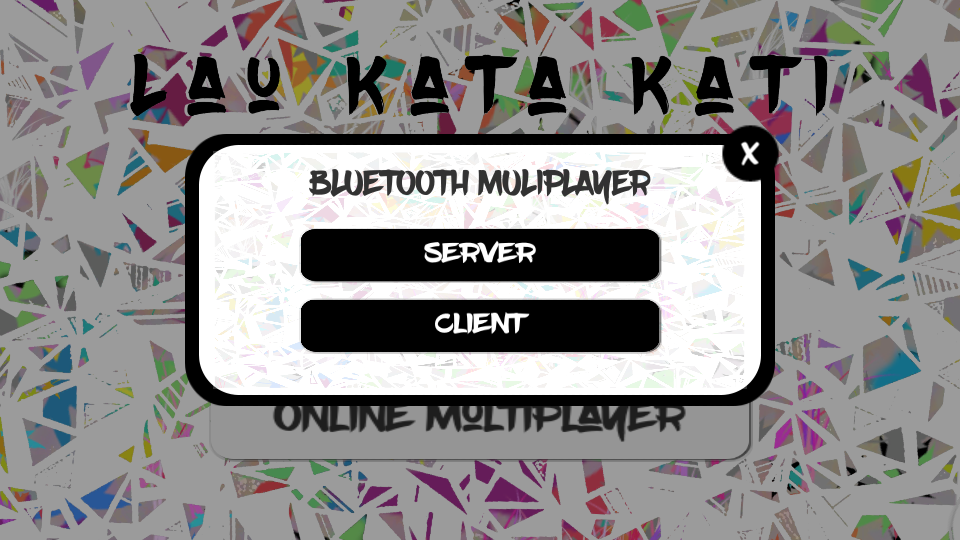
\includegraphics[width=55mm]{img/bluetooth.png}
		\caption{Opcje trybu Online multiplayer}
	\end{figure}
\end{enumerate}		% instrukcja uzytkowania aplikacji
\section{Podsumowanie}
Pomimo napotkanych błędów wszystkie założenia projektu zostały zrealizowane pomyślnie.\\
Projekt jest wrat kontynuacji. Możliwości jego rozwoju są wręcz nieograniczone. Główny rdzeń aplikacji jest przygotowany do kolejnych rozszerzeń, co zawdzięczamy architekturze MVC.

Przykładowe kierunki rozwoju:
\begin{itemize}
	\item Rozgrywka sieciowa
	\item Parowanie urzadzeń za pomocą NFC
	\item Ranking graczy
	\item Nowe skórki pionków
	\item Skórki plansz
\end{itemize}	% podsumowanie i wnioski
\newpage\listoffigures
  \addcontentsline{toc}{section}{Spis rysunków}
\listoftables
  \addcontentsline{toc}{section}{Spis tabel}			% spis rysunków i tabel
\end{document}